% AI Agent Harness Architecture and Engineering Guide
% Standalone, editable LaTeX source. Compile: latexmk -pdf -interaction=nonstopmode file.tex
\documentclass[10pt,letterpaper]{article}
\usepackage[T1]{fontenc}
\usepackage[utf8]{inputenc}
\usepackage{lmodern}
\usepackage{microtype}
\usepackage[margin=0.83in,headheight=16pt,headsep=13pt,footskip=24pt]{geometry}
\usepackage[table]{xcolor}
\usepackage{graphicx}
\usepackage{tikz}
\usetikzlibrary{arrows.meta,positioning,calc,shapes.geometric,fit}
\usepackage[most]{tcolorbox}
\usepackage{booktabs,tabularx,longtable,array,multirow}
\usepackage{enumitem}
\usepackage{listings}
\usepackage{caption}
\usepackage{fancyhdr}
\usepackage{titlesec}
\usepackage{hyperref}
\usepackage{xurl}
\usepackage{needspace}
\usepackage{float}
\usepackage{amsmath,amssymb}
\usepackage{lastpage}

% ---------- Design tokens ----------
\definecolor{Navy}{HTML}{10223D}
\definecolor{DeepBlue}{HTML}{17365D}
\definecolor{Ocean}{HTML}{2869A7}
\definecolor{Teal}{HTML}{078989}
\definecolor{PaleBlue}{HTML}{EDF4FA}
\definecolor{PaleTeal}{HTML}{EDF9F7}
\definecolor{PaleAmber}{HTML}{FFF6E6}
\definecolor{Amber}{HTML}{B97C24}
\definecolor{Slate}{HTML}{42536B}
\definecolor{CoolGray}{HTML}{E1E7EF}
\definecolor{PaperGray}{HTML}{F6F8FB}
\definecolor{Ink}{HTML}{182536}
\definecolor{CodeBg}{HTML}{F4F7FB}
\definecolor{CodeComment}{HTML}{63738A}
\color{Ink}

\hypersetup{
  colorlinks=true,
  linkcolor=Ocean,
  urlcolor=Ocean,
  citecolor=Teal,
  pdftitle={AI Agent Harness: Architecture and Engineering Guide},
  pdfauthor={Engineering Reference},
  pdfsubject={Architecture, operational controls, reference control loop, and evaluation plan for coding agents},
  pdfkeywords={AI agents, harness, context compaction, MCP, safety, verification, coding agents}
}
\urlstyle{same}
\setlength{\parindent}{0pt}
\setlength{\parskip}{6pt}
\setlist[itemize]{leftmargin=1.35em, itemsep=2pt, topsep=3pt}
\setlist[enumerate]{leftmargin=1.55em, itemsep=3pt, topsep=3pt}
\renewcommand{\arraystretch}{1.2}
\captionsetup{font=small,labelfont={bf,color=DeepBlue},textfont={color=Slate}}

\titleformat{\section}{\Large\bfseries\color{Navy}}{\thesection}{0.65em}{}[\vspace{-4pt}\color{CoolGray}\titlerule]
\titleformat{\subsection}{\large\bfseries\color{DeepBlue}}{\thesubsection}{0.55em}{}
\titleformat{\subsubsection}{\normalsize\bfseries\color{Teal}}{\thesubsubsection}{0.55em}{}
\titlespacing*{\section}{0pt}{20pt}{11pt}
\titlespacing*{\subsection}{0pt}{12pt}{5pt}
\titlespacing*{\subsubsection}{0pt}{9pt}{3pt}

\pagestyle{fancy}
\fancyhf{}
\fancyhead[L]{\footnotesize\sffamily\color{Slate} AI AGENT HARNESS / ENGINEERING GUIDE}
\fancyhead[R]{\footnotesize\sffamily\color{Ocean}\nouppercase{\leftmark}}
\fancyfoot[L]{\scriptsize\color{Slate} Reference architecture \textbullet\ November 2026}
\fancyfoot[R]{\scriptsize\color{Slate} \thepage\ / \pageref{LastPage}}
\renewcommand{\headrulewidth}{0.4pt}
\renewcommand{\footrulewidth}{0pt}

\newtcolorbox{summarybox}[1][]{enhanced,breakable,colback=PaleBlue,colframe=Ocean,boxrule=0.65pt,arc=2mm,left=11pt,right=11pt,top=10pt,bottom=9pt,#1}
\newtcolorbox{principlebox}[1][]{enhanced,breakable,colback=PaleTeal,colframe=Teal,boxrule=0.65pt,arc=2mm,left=10pt,right=10pt,top=9pt,bottom=8pt,#1}
\newtcolorbox{riskbox}[1][]{enhanced,breakable,colback=PaleAmber,colframe=Amber,boxrule=0.65pt,arc=2mm,left=10pt,right=10pt,top=9pt,bottom=8pt,#1}
\newcommand{\term}[1]{\textbf{\color{DeepBlue}#1}}
\newcommand{\code}[1]{\texttt{#1}}
\newcommand{\smallcaplabel}[1]{\textsf{\bfseries\footnotesize\color{Ocean}\MakeUppercase{#1}}}
\newcolumntype{Y}{>{\raggedright\arraybackslash}X}
\newcolumntype{L}[1]{>{\raggedright\arraybackslash}p{#1}}

\lstdefinestyle{harnesscode}{
  backgroundcolor=\color{CodeBg},
  basicstyle=\ttfamily\footnotesize,
  keywordstyle=\color{Ocean}\bfseries,
  commentstyle=\color{CodeComment}\itshape,
  stringstyle=\color{Teal},
  numbers=left,
  numberstyle=\tiny\color{Slate},
  numbersep=8pt,
  stepnumber=1,
  breaklines=true,
  breakatwhitespace=false,
  frame=single,
  rulecolor=\color{CoolGray},
  frameround=tttt,
  xleftmargin=1.2em,
  framexleftmargin=0.8em,
  framesep=7pt,
  showstringspaces=false,
  keepspaces=true,
  tabsize=4,
  postbreak=\mbox{\textcolor{Ocean}{$\hookrightarrow$}\space},
  captionpos=b,
  aboveskip=10pt,
  belowskip=10pt
}
\lstdefinestyle{pythonstyle}{style=harnesscode,language=Python,morekeywords={Protocol,dataclass,field,Any,Sequence}}
\lstdefinestyle{textstyle}{style=harnesscode,language={},numbers=none}
\lstdefinestyle{yamlstyle}{style=harnesscode,language={},numbers=none,morecomment=[l]{\#}}

\begin{document}
\hypersetup{pageanchor=false}

% ---------- Cover ----------
\thispagestyle{empty}
\begin{tikzpicture}[remember picture,overlay]
  \fill[Navy] (current page.north west) rectangle ([xshift=17mm]current page.south west);
  \fill[Ocean] ([xshift=17mm]current page.north west) rectangle ([xshift=20mm]current page.south west);
  \fill[PaperGray] ([yshift=-33mm,xshift=20mm]current page.north west) rectangle ([yshift=-35mm]current page.north east);
  \draw[Ocean!24,line width=1.7pt] ([xshift=-24mm,yshift=-64mm]current page.north east) circle (28mm);
  \draw[Teal!31,line width=1pt] ([xshift=-26mm,yshift=-64mm]current page.north east) circle (19mm);
  \fill[Ocean!70] ([xshift=-40mm,yshift=-59mm]current page.north east) circle (2.7mm);
  \fill[Teal] ([xshift=-13mm,yshift=-76mm]current page.north east) circle (2.1mm);
\end{tikzpicture}
\vspace*{27mm}
\hspace*{7mm}{\smallcaplabel{Systems engineering / Reference architecture}}\\[17mm]
\hspace*{7mm}{\parbox{0.88\textwidth}{\fontsize{32}{38}\selectfont\bfseries\color{Navy}AI Agent Harness\\Architecture \&\\Engineering Guide}}\\[9mm]
\hspace*{7mm}{\parbox{0.82\textwidth}{\large\color{Slate}Building a repository-aware coding agent with bounded execution, context compaction, enforceable security controls, and evidence-driven verification.}}\\[24mm]
\hspace*{7mm}{\begin{minipage}{0.83\textwidth}
\begin{tcolorbox}[colback=PaleBlue,colframe=CoolGray,boxrule=0.5pt,arc=1.5mm,left=13pt,right=13pt,top=12pt,bottom=12pt]
\textbf{Design objective}\par
Turn an LLM from a text-generating component into a controlled software-engineering worker that can inspect a repository, propose and apply changes, test its work, recover from failure, and report verifiable evidence.
\end{tcolorbox}
\end{minipage}}
\vfill
\hspace*{7mm}{\begin{minipage}{0.85\textwidth}
\color{Slate}\footnotesize
\textbf{Edition:} 1.0 \quad\textbf{Date:} November 2026\\
\textbf{Audience:} Software engineers, platform engineers, AI/agent engineers, application-security engineers\\
\textbf{Format:} Self-contained LaTeX with editable vector diagrams and code listings
\end{minipage}}
\vspace*{11mm}
\clearpage

% ---------- Contents ----------
\hypersetup{pageanchor=true}
\pagenumbering{arabic}
\setcounter{page}{1}
\begingroup
\small
\setlength{\parskip}{0pt}
\tableofcontents
\endgroup
\clearpage
\vspace{3mm}
\begin{summarybox}
\smallcaplabel{Executive summary}\par
An \term{AI agent harness} is the runtime infrastructure around a language model. It assembles instructions and context, coordinates an iterative decision loop, brokers tool access, manages state, enforces permissions, and verifies outcomes. The LLM can \emph{propose} actions; the harness must \emph{decide whether and how those actions are executed}. This guide presents a practical reference architecture for a repository-aware software-engineering agent and a phased path from prototype to dependable operation.
\end{summarybox}
\vspace{4mm}
\textbf{Reader's path.} Start with the system diagram (Section~\ref{sec:architecture}), use the eight-component specification (Section~\ref{sec:components}) as a design checklist, implement the runtime contract (Section~\ref{sec:loop}), then apply the security and verification gates (Sections~\ref{sec:security}--\ref{sec:evaluation}).
\medskip

\section{Purpose, Scope, and Design Principles}\label{sec:purpose}
\subsection{Problem statement}
A raw language model generates responses from its input context. It does not, by itself, guarantee state continuity, access control, reliable execution, bounded resource consumption, or truthful claims about completed work. The harness supplies those system-level properties through explicit orchestration and independently observable outputs.

\subsection{Target use case: repository-aware coding agent}
The target agent accepts a software-engineering task (for example, a GitHub issue) and, within an approved repository and environment, can discover project conventions, inspect code, create a scoped change, run relevant checks, and produce a reviewable patch or pull request. A successful result includes both the changed artifacts and evidence that the acceptance criteria were evaluated.

\begin{principlebox}
\textbf{Core engineering rule:} Instructions such as \code{AGENTS.md} guide agent behavior, but they are not a security boundary. Access restrictions must be implemented by the tool broker, operating-system sandbox, credentials, network controls, and approval workflow.
\end{principlebox}

\subsection{Non-negotiable design properties}
\begin{itemize}
  \item \term{Bounded:} enforce maximum steps, elapsed time, tool calls, and model/tool budgets.
  \item \term{Least privilege:} restrict file paths, processes, network targets, secrets, and identity scopes.
  \item \term{Auditable:} retain tool requests, policy decisions, results, verification, and source commit IDs.
  \item \term{Recoverable:} checkpoint durable task state and make retries safe and idempotent where feasible.
  \item \term{Verifiable:} compare outputs against independently executed acceptance checks.
  \item \term{Reviewable:} keep changes isolated and require human approval for sensitive mutations or merges.
\end{itemize}

\Needspace{24\baselineskip}
\section{Reference System Architecture}\label{sec:architecture}
\begin{figure}[H]
\centering
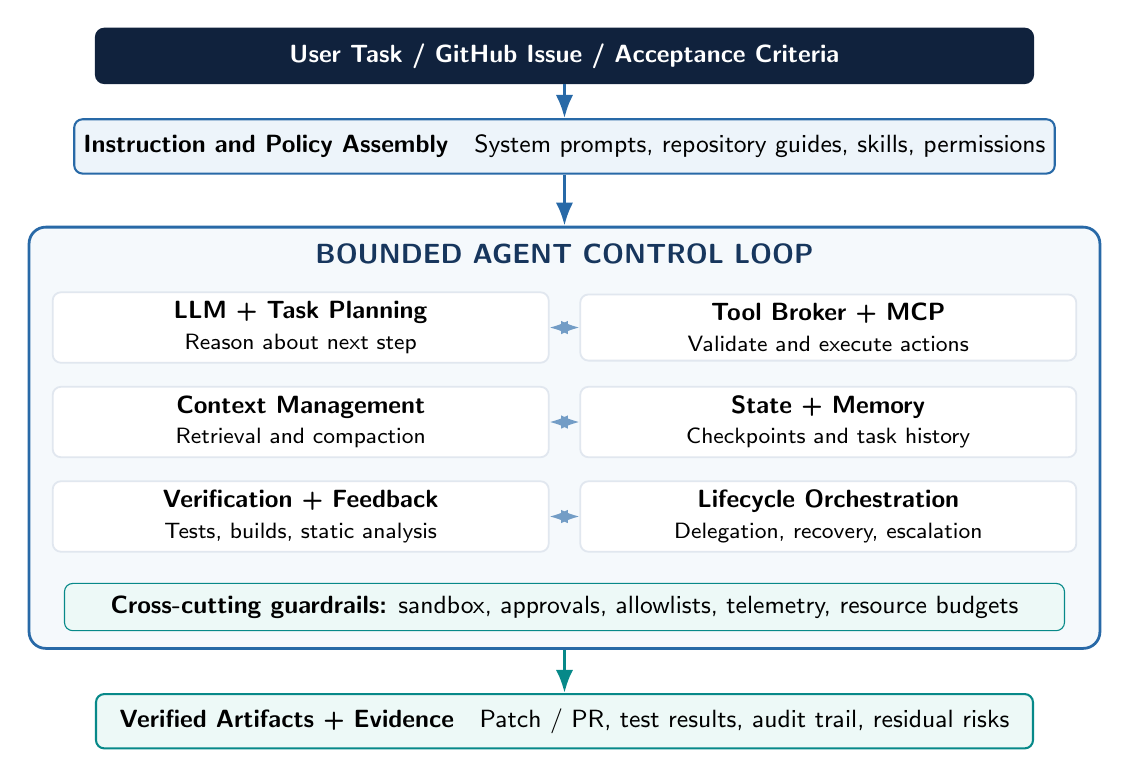
\begin{tikzpicture}[>=Latex, font=\sffamily\small,
  stack/.style={draw=Ocean,rounded corners=3pt,minimum width=11.9cm,minimum height=0.69cm,align=center,fill=PaleBlue,line width=.75pt},
  cell/.style={draw=CoolGray,rounded corners=3pt,minimum width=6.3cm,minimum height=0.76cm,align=center,fill=white,line width=.65pt},
  outer/.style={draw=Ocean,rounded corners=6pt,fill=PaleBlue!55,minimum width=13.6cm,minimum height=5.35cm,line width=1pt}]
  \node[stack, fill=Navy, draw=Navy, text=white] (task) at (0,5.2) {\textbf{User Task / GitHub Issue / Acceptance Criteria}};
  \node[stack] (instruction) at (0,4.05) {\textbf{Instruction and Policy Assembly}\quad System prompts, repository guides, skills, permissions};
  \node[outer] (harness) at (0,0.35) {};
  \node[font=\sffamily\bfseries\color{DeepBlue}] at (0,2.68) {BOUNDED AGENT CONTROL LOOP};
  \node[cell] (model) at (-3.35,1.75) {\textbf{LLM + Task Planning}\\\footnotesize Reason about next step};
  \node[cell] (tools) at (3.35,1.75) {\textbf{Tool Broker + MCP}\\\footnotesize Validate and execute actions};
  \node[cell] (context) at (-3.35,0.55) {\textbf{Context Management}\\\footnotesize Retrieval and compaction};
  \node[cell] (state) at (3.35,0.55) {\textbf{State + Memory}\\\footnotesize Checkpoints and task history};
  \node[cell] (verify) at (-3.35,-0.65) {\textbf{Verification + Feedback}\\\footnotesize Tests, builds, static analysis};
  \node[cell] (orchestration) at (3.35,-0.65) {\textbf{Lifecycle Orchestration}\\\footnotesize Delegation, recovery, escalation};
  \node[draw=Teal,fill=PaleTeal,rounded corners=3pt,minimum width=12.7cm,minimum height=.60cm,align=center] (guard) at (0,-1.8) {\textbf{Cross-cutting guardrails:} sandbox, approvals, allowlists, telemetry, resource budgets};
  \node[stack, fill=PaleTeal, draw=Teal] (result) at (0,-3.25) {\textbf{Verified Artifacts + Evidence}\quad Patch / PR, test results, audit trail, residual risks};
  \draw[->,very thick,Ocean] (task) -- (instruction);
  \draw[->,very thick,Ocean] (instruction) -- (harness.north);
  \draw[->,very thick,Teal] (harness.south) -- (result.north);
  \draw[<->,thick,Ocean!65] (model.east) -- (tools.west);
  \draw[<->,thick,Ocean!65] (context.east) -- (state.west);
  \draw[<->,thick,Ocean!65] (verify.east) -- (orchestration.west);
\end{tikzpicture}
\caption{Logical reference architecture. Controls are cross-cutting; the diagram shows responsibilities, not mandatory service boundaries.}
\label{fig:architecture}
\end{figure}

\subsection{Boundary and ownership model}
\begin{tabularx}{\textwidth}{L{2.75cm} Y Y}
\toprule
\textbf{Layer} & \textbf{Owns} & \textbf{Must not assume} \\
\midrule
LLM & Reasoning proposals, tool intents, candidate responses & Permission to execute, ground-truth success, durable memory \\
Harness & Loop, state, budgets, routing, approvals, observations & That model outputs are authoritative \\
Tool broker & Schema validation, policy checks, scoped execution & That well-formed calls are inherently safe \\
Execution sandbox & Process isolation, files, network, credentials & That instructions embedded in content are trusted \\
Verification system & Objective checks and evidence collection & That the model's self-evaluation is sufficient \\
Human / policy owner & High-risk approvals, scope changes, merge decisions & That autonomy removes accountability \\
\bottomrule
\end{tabularx}

\section{Eight Core Harness Components}\label{sec:components}
\subsection{Agent and control loop}
The control loop repeatedly sends a bounded context to the model, interprets its next action, executes permitted tools, records observations, and checks for termination. Its responsibilities include terminal-state detection, cancellation, retries, step limits, and clear distinctions between \emph{finished}, \emph{blocked}, and \emph{budget exhausted}.

\textbf{Interface:} \code{next(model\_context) -> final\_answer | tool\_calls}.\\
\textbf{Failure mode:} infinite retry or falsely reporting a task as complete.\\
\textbf{Control:} enforce explicit budgets and terminal-state reasons.

\subsection{System prompt and repository guide assembly}
Instruction assembly combines trusted system/developer policy, task instructions, project conventions, relevant skills, and a focused repository map. Files such as \code{AGENTS.md} and other project-specific guides can direct build and style conventions but must be treated as source-scoped guidance rather than authorization.

\textbf{Inputs:} trusted policy, task requirements, discovered repository guidance.\\
\textbf{Failure mode:} prompt injection or competing instructions override security policy.\\
\textbf{Control:} maintain instruction provenance and deterministic precedence.

\subsection{Tools and tool dispatch}
The tool broker translates structured model tool requests into controlled actions. Typical adapters provide repository reads, diff application, Git operations, shell execution in a sandbox, test invocation, and Model Context Protocol (MCP) access.

\textbf{Inputs:} typed tool name, validated arguments, authorization context.\\
\textbf{Outputs:} status, structured result, bounded log reference, duration.\\
\textbf{Control:} schema validation, allowlists, path normalization, execution timeouts, and policy decisions before side effects.

\subsection{Context management and compaction}
A context manager selects only material information for the current decision: user intent, repository facts, relevant code spans, recent observations, and outstanding acceptance criteria. Compaction should preserve operational meaning while reducing token usage.

\textbf{Techniques:} retrieval, deduplication, summary checkpoints, truncation, artifact references, progressive skill disclosure.\\
\textbf{Failure mode:} removing a crucial requirement or error and causing repeated or unsafe changes.\\
\textbf{Control:} preserve a non-compacting task specification and attach provenance to compressed observations.

\subsection{State and memory management}
Separate \term{working context} (model-visible material), \term{session state} (current plan, tool results, budgets), and \term{durable memory} (reusable facts and task artifacts). Checkpoints store enough information to resume safely; durable Git commits and logs provide an external record, not a substitute for explicit task state.

\textbf{Control:} stable run IDs, checkpoint versioning, task-state transitions, data retention and access policies.

\subsection{Verification and feedback loops}
Verification executes trusted commands outside the model's narrative: linters, test suites, build pipelines, type checkers, policy scanners, and change-specific assertions. Failures become observations for repair, while evidence links to the exact source revision.

\textbf{Control:} record the command, environment, exit code, logs, commit SHA, and relevant acceptance criterion; never turn incomplete checks into a success claim.

\subsection{Guardrails and permissions}
Defense in depth includes authorization policy, filesystem scoping, process isolation, network egress controls, secret handling, command approval, rate limits, data classification, and audit events. Human approval may be mandatory for sensitive operations regardless of the model's confidence.

\textbf{Control:} enforce decisions externally to the LLM; fail closed when the authorization decision is unavailable.

\subsection{Sub-agents and lifecycle orchestration}
Specialized agents may independently research code, generate tests, or review a proposed diff. Orchestration owns delegation contracts, budget allocation, artifact handoff, retries, cancellation, and escalation. A single-agent harness is generally the first reliable baseline against which delegation should be measured.

\textbf{Control:} apply the same authorization and observability rules to every child agent; never allow privilege expansion through delegation.

\section{Runtime Contract and Bounded Control Loop}\label{sec:loop}
\subsection{Suggested state machine}
\begin{figure}[H]
\centering
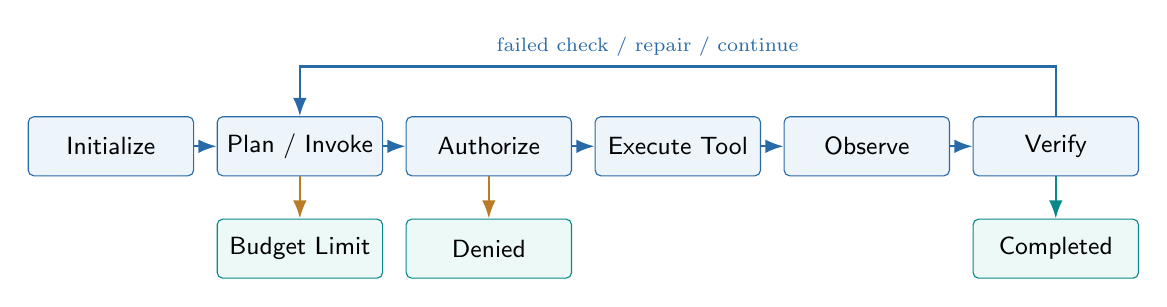
\begin{tikzpicture}[>=Latex, font=\sffamily\small,
  state/.style={draw=Ocean,fill=PaleBlue,rounded corners=2pt,minimum width=2.1cm,minimum height=.75cm,align=center},
  terminal/.style={draw=Teal,fill=PaleTeal,rounded corners=2pt,minimum width=2.1cm,minimum height=.75cm,align=center}]
\node[state] (init) at (-6.0,0) {Initialize};
\node[state] (plan) at (-3.6,0) {Plan / Invoke};
\node[state] (authorize) at (-1.2,0) {Authorize};
\node[state] (execute) at (1.2,0) {Execute Tool};
\node[state] (observe) at (3.6,0) {Observe};
\node[state] (verify) at (6.0,0) {Verify};
\node[terminal] (expired) at (-3.6,-1.3) {Budget Limit};
\node[terminal] (blocked) at (-1.2,-1.3) {Denied};
\node[terminal] (completed) at (6.0,-1.3) {Completed};
\draw[->,thick,Ocean] (init)--(plan);
\draw[->,thick,Ocean] (plan)--(authorize);
\draw[->,thick,Ocean] (authorize)--(execute);
\draw[->,thick,Ocean] (execute)--(observe);
\draw[->,thick,Ocean] (observe)--(verify);
\draw[->,thick,Amber] (plan)--(expired);
\draw[->,thick,Amber] (authorize)--(blocked);
\draw[->,thick,Teal] (verify)--(completed);
\draw[->,thick,Ocean] (verify.north) -- ++(0,.63) -| node[pos=.27,above,font=\scriptsize]{failed check / repair / continue} (plan.north);
\end{tikzpicture}
\caption{Illustrative lifecycle. Explicit denial and budget terminal states prevent false-positive completion.}
\end{figure}

\subsection{Reference loop (Python-style pseudocode)}
The following is deliberately illustrative. The implementation must provide real adapters for model inference, tool execution, checkpoint storage, and verification.
\begin{lstlisting}[style=pythonstyle,caption={Bounded agent orchestration pseudocode.}]
def run_agent(task, model, broker, verifier, store, limits):
    state = store.start(task=task, status="running")

    while state.steps < limits.max_steps:
        if limits.deadline_exceeded() or limits.cost_exceeded():
            return store.finish(state, status="budget_exhausted")

        context = assemble_context(
            task=task,
            checkpoint=state,
            token_budget=limits.context_tokens,
        )
        turn = model.next(context)
        state.steps += 1

        if turn.final_answer is not None:
            result = verifier.check(task, state.workspace)
            store.record_verification(state, result)
            if result.passed:
                return store.finish(state, status="completed",
                                    answer=turn.final_answer)
            state.observations.append(result.summary)
            store.checkpoint(state)
            continue

        for call in turn.tool_calls:
            decision = broker.authorize(call, state.identity)
            if not decision.allowed:
                state.observations.append(decision.explanation)
                continue
            observation = broker.execute(
                call, timeout=limits.tool_timeout
            )
            state.observations.append(
                persist_and_summarize(observation, store)
            )
        store.checkpoint(state)

    return store.finish(state, status="step_limit")
\end{lstlisting}

\begin{riskbox}
\textbf{Implementation note.} A model-generated \code{final\_answer} is not sufficient evidence of success. Completion should require the task-specific verification policy to pass. A budget-exhausted or denied run must report partial artifacts and the reason it stopped.
\end{riskbox}

\subsection{Key data contracts}
\begin{tabularx}{\textwidth}{L{3.0cm} Y}
\toprule
\textbf{Object} & \textbf{Essential fields} \\
\midrule
\code{TaskSpec} & Request, repository ID, base commit SHA, scope, acceptance criteria, risk class \\
\code{RunState} & Run ID, phase/status, step counter, budgets, active branch, checkpoint version \\
\code{ToolCall} & Typed tool name, validated arguments, caller identity, correlation ID \\
\code{ToolResult} & Exit status, elapsed time, output/artifact reference, truncation flag \\
\code{PolicyDecision} & Allow / deny / approve, governing rule, principal, decision timestamp \\
\code{VerifyRecord} & Check name, command, source SHA, environment, status, evidence URI \\
\code{FinalReport} & Change summary, verification, limitations, remaining risks, artifact links \\
\bottomrule
\end{tabularx}

\section{Context Engineering and Compaction}\label{sec:context}
\subsection{A three-tier context model}
\begin{enumerate}
\item \term{Immutable task kernel.} Original request, acceptance criteria, branch/repository scope, authorization constraints, and explicit user decisions. Never silently replace these with a summary.
\item \term{Active working set.} Relevant code slices, current plan, latest model/tool turns, failing tests, and next actions. Refresh based on task phase.
\item \term{External artifact store.} Large logs, full diffs, previous observations, generated files, and checkpoints, referenced by stable IDs with retrieval support.
\end{enumerate}

\subsection{Compaction pipeline}
\begin{figure}[H]
\centering
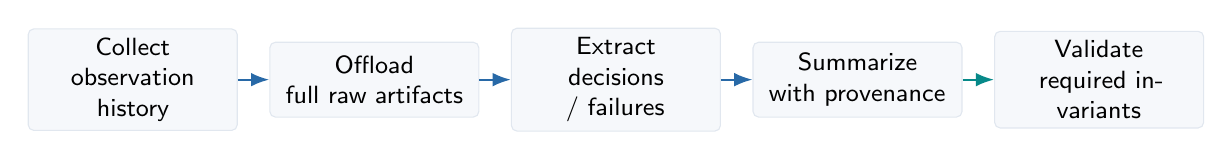
\begin{tikzpicture}[>=Latex, node distance=4mm, font=\sffamily\small,
    stage/.style={draw=CoolGray,fill=PaperGray,rounded corners=2pt,align=center,minimum height=.95cm,text width=2.42cm}]
\node[stage] (collect) {Collect\\observation history};
\node[stage,right=of collect] (offload) {Offload\\full raw artifacts};
\node[stage,right=of offload] (select) {Extract\\decisions / failures};
\node[stage,right=of select] (summ) {Summarize\\with provenance};
\node[stage,right=of summ] (validate) {Validate\\required invariants};
\draw[->,thick,Ocean] (collect)--(offload);
\draw[->,thick,Ocean] (offload)--(select);
\draw[->,thick,Ocean] (select)--(summ);
\draw[->,thick,Teal] (summ)--(validate);
\end{tikzpicture}
\caption{Compaction reduces model-visible tokens without erasing the full underlying evidence.}
\end{figure}

\begin{summarybox}
\textbf{Required compaction invariants}\par
A compacted state must preserve: (1) the task objective and acceptance criteria; (2) approved/denied boundaries; (3) changes already made and their source revisions; (4) outstanding errors and unresolved decisions; (5) next actions; and (6) references to underlying logs. Summaries should be tagged as summaries, not raw evidence.
\end{summarybox}

\subsection{Context quality checks}
For a sample of tasks, compare full-history and compacted-history continuation against the same acceptance criteria. Track omission defects, repeated tool calls, token usage, recovery behavior, and unauthorized-action attempts. A smaller context is not an improvement if it loses important task state.

\section{Security, Permissions, and Trust Boundaries}\label{sec:security}
\subsection{Trust model}
Treat repository files, issues, web pages, tool outputs, dependency metadata, and external MCP responses as \term{untrusted data}. They may contain malicious or irrelevant instructions. The model may analyze that content, but the harness must not promote it into privileged system policy or allow it to expand tool scope.

\subsection{Control catalog}
\begin{longtable}{L{3.15cm} L{5.6cm} L{6.0cm}}
\toprule
\textbf{Threat / failure} & \textbf{Control} & \textbf{Verification evidence} \\
\midrule
\endfirsthead
\toprule
\textbf{Threat / failure} & \textbf{Control} & \textbf{Verification evidence} \\
\midrule
\endhead
Prompt injection & Instruction provenance, untrusted-content delimiters, immutable policy, tool-side authorization & Red-team corpus; denied escalation attempts \\
Unsafe command & Command/argument validation, sandbox, process permissions, timeouts & Command policy tests; sandbox logs \\
Path traversal & Canonical path validation, workspace root constraints, restricted mounts & Negative tests using \code{../} and symlink paths \\
Secret exfiltration & Secret isolation, scoped short-lived credentials, network egress policy & Credential scope review; blocked egress test \\
Unreviewed code merge & Branch protection, required CI, human approval where required & Pull-request rules and approval/audit events \\
Resource exhaustion & Tool/model/step budgets, concurrency limits, cancellation & Budget-exhaustion scenarios \\
False success & Independent assertions, source-SHA-bound test evidence & Reproducible verification records \\
Delegated privilege abuse & Child-agent policy inheritance, scoped tool identities & Permission tests across parent/child boundaries \\
\bottomrule
\end{longtable}

\subsection{Illustrative policy configuration}
This is a \emph{design sketch}, not a plug-and-play policy file for a specific enforcement engine. Actual enforcement must occur in the broker and runtime environment.
\begin{lstlisting}[style=yamlstyle,caption={Illustrative execution policy for a repository coding agent.}]
agent:
  mode: coding
  max_steps: 40
  max_tool_seconds: 120
  max_parallel_subagents: 0  # first release
workspace:
  root: /workspace/repository
  allowed_write_paths:
    - src/
    - tests/
    - docs/
  denied_paths:
    - .git/objects/
    - .env
    - secrets/
tools:
  allow: [repo_read, diff_apply, git_status, test_runner]
  require_approval: [network_write, publish, merge, secret_access]
execution:
  network_egress: deny_by_default
  sandbox: required
  fail_closed_on_policy_error: true
verification:
  require: [lint, tests, build]
  bind_to_source_commit: true
\end{lstlisting}

\section{Verification, Observability, and Evaluation}\label{sec:evaluation}
\subsection{Verification pipeline}
Every completed coding task should generate a change-specific verification report. The baseline pipeline is \term{format/lint} $\rightarrow$ \term{type/static checks} $\rightarrow$ \term{tests} $\rightarrow$ \term{build} $\rightarrow$ \term{security checks}, where applicable. Tests must match the language and build system detected in the actual repository rather than a hardcoded universal command.

\subsection{Key measures}
\begin{tabularx}{\textwidth}{L{3.5cm} Y L{3.25cm}}
\toprule
\textbf{Metric} & \textbf{Definition} & \textbf{Why it matters} \\
\midrule
Verified task success & Passed acceptance criteria / attempted eligible tasks & Outcome reliability \\
Policy violation rate & Unauthorized actions actually executed / total runs & Security effectiveness \\
Blocked unsafe intents & Unauthorized actions denied by policy / total denied attempts & Guardrail coverage \\
Repair efficiency & Verified fixes / repair cycles & Loop quality \\
Median task cost & Model + tool cost per completed run & Economic efficiency \\
Context efficiency & Tokens used per verified completion, with error rates & Compaction quality \\
Recovery success & Interrupted runs resumed to verified termination / resumptions & Durability \\
Human intervention & Approvals and escalations per task class & Operational workload \\
\bottomrule
\end{tabularx}

\subsection{Minimum audit event}
For each tool execution retain \code{run\_id}, \code{task\_id}, tool name, validated arguments or redacted representation, principal, decision, workspace identifier, commit SHA, duration, status, and artifact reference. Redact credentials and sensitive data before logging; observe the retention and access policies relevant to the organization.

\section{Phased Implementation Roadmap}\label{sec:roadmap}
\small
\begin{longtable}{L{2.0cm} L{3.5cm} L{5.0cm} L{4.2cm}}
\toprule
\textbf{Phase} & \textbf{Deliverable} & \textbf{Acceptance test} & \textbf{Primary risk addressed} \\
\midrule
\endfirsthead
\toprule
\textbf{Phase} & \textbf{Deliverable} & \textbf{Acceptance test} & \textbf{Primary risk addressed} \\
\midrule
\endhead
01 Foundation & Model adapter, explicit state machine, bounded loop & Halts correctly for completion, denial, cancellation, and each budget limit & Infinite loops and false completion \\
02 Tools & Broker with sandboxed Git, filesystem, shell and optional MCP adapters & Allowed calls work; forbidden commands and paths fail closed & Uncontrolled side effects \\
03 Repository context & Build-system detection, repo map, guides, scoped retrieval & Discovers actual build/test commands and respects task scope & Incorrect assumptions about codebase \\
04 Context & Retrieval, artifact offloading, compaction/checkpoints & Continuation preserves all required invariants & Context loss and repeated work \\
05 Verification & Lint, test, build, static/security check runners & Evidence tied to exact source SHA and acceptance criteria & Unverified code changes \\
06 Persistence & Durable run store, checkpointing, safe resume & Forced interruption resumes without duplicate destructive actions & Fragile long-running tasks \\
07 Orchestration & Specialized sub-agents and lifecycle hooks & Delegated tools cannot exceed parent policy; measured benefit & Coordination / privilege expansion \\
08 Evaluation & Benchmarks, dashboards, audit reports & Reproducible success, failure, cost, and safety metrics & Inability to improve or govern \\
\bottomrule
\end{longtable}
\normalsize

\subsection{Recommended initial technology choices}
\begin{tabularx}{\textwidth}{L{3.2cm} Y}
\toprule
\textbf{Concern} & \textbf{Starting choice and rationale} \\
\midrule
Harness runtime & Python 3.11+ for rapid adapter development and testability; language-independent protocol boundaries \\
Tools and integrations & Explicit typed tool registry; MCP adapters where interoperability adds value \\
Isolation & Ephemeral container/worktree per task with restrictive mounts and egress \\
Durable artifacts & Git for code history; object/file store for full logs and test artifacts \\
State and checkpoints & Structured durable store with schema versioning and stable run IDs \\
Independent CI & GitHub Actions or equivalent to verify a candidate branch separately from the agent \\
Observability & Structured events, traces, cost counters, redacted tool logs \\
\bottomrule
\end{tabularx}

\section{First Practical Laboratory: Issue to Verified Patch}\label{sec:lab}
\smallcaplabel{Laboratory objective}\par
Implement a bounded coding agent that handles one repository issue and produces a tested change set without granting merge or publication privileges.

\subsection{Environment and prerequisites}
Use a disposable repository or a protected test branch; install the repository's actual language toolchain, a container runtime, and Git. Provide an issue with precise acceptance criteria, a known failing test, and a clearly scoped set of editable paths.

\subsection{Lab procedure}
\begin{enumerate}
  \item \textbf{Inspect:} identify repository root, tracked files, guides, dependency manifests, CI checks, and current commit SHA.
  \item \textbf{Plan:} produce a proposed file/change map, required tests, and tool budget; explicitly record unresolved assumptions.
  \item \textbf{Branch:} create an isolated worktree or task branch from the approved base revision.
  \item \textbf{Edit:} apply a minimal diff through the authorized tool broker; record changed files and tool outcomes.
  \item \textbf{Verify:} run unit tests, lint/static analysis, and build commands that are applicable to the repository.
  \item \textbf{Repair:} feed failed checks back as observations within the remaining budget; do not suppress failing evidence.
  \item \textbf{Report:} emit a change summary, resulting commit SHA, tests and statuses, evidence references, and any remaining limitations.
  \item \textbf{Review:} stop at a reviewable patch or draft pull request; keep protected-branch merge outside this first lab.
\end{enumerate}

\subsection{Acceptance criteria}
\begin{tcolorbox}[colback=PaperGray,colframe=CoolGray,breakable,arc=1.5mm,title={\color{DeepBlue}\bfseries Definition of done}]
\begin{itemize}[label=$\square$]
  \item The agent modifies only approved paths in an isolated worktree/branch.
  \item Every external tool invocation is recorded and policy checked.
  \item The task ends in an explicit terminal state rather than an unbounded loop.
  \item Required checks are independently executed; failures are not disguised as passes.
  \item Verification results identify the source commit that was tested.
  \item Interrupted runs can resume from a checkpoint without replaying unsafe operations.
  \item The final report includes artifacts, evidence, residual risks, and unresolved issues.
\end{itemize}
\end{tcolorbox}

\subsection{Suggested repository layout}
\begin{lstlisting}[style=textstyle,caption={Minimal harness project structure.}]
agent-harness/
  pyproject.toml
  README.md
  policies/
    execution-policy.yaml
  src/harness/
    control_loop.py
    state.py
    context.py
    compaction.py
    tool_broker.py
    policy.py
    verification.py
    audit.py
    adapters/
      model.py
      git.py
      shell.py
      mcp.py
  tests/
    test_budget_limits.py
    test_policy_denials.py
    test_compaction_invariants.py
    test_checkpoint_resume.py
    test_verification_evidence.py
  examples/
    sample_issue.md
    AGENTS.md
\end{lstlisting}

\section{Architecture Decision Checklist}\label{sec:adr}
Before extending beyond the first lab, record decisions for the following questions in architecture decision records (ADRs):
\begin{enumerate}
  \item \term{Control flow:} which terminal states and retries are supported, and who sets budgets?
  \item \term{Trust hierarchy:} how are trusted instructions distinguished from repository and tool data?
  \item \term{Execution boundary:} what process, filesystem, credential, and network constraints apply?
  \item \term{Context provenance:} what is summarized, what stays immutable, and how is raw evidence retrieved?
  \item \term{Persistence:} which checkpoints survive restarts, and how are schema migrations handled?
  \item \term{Verification:} what qualifies as success, and what evidence must be attached?
  \item \term{Human authority:} which actions require approval and which are explicitly forbidden?
  \item \term{Delegation:} when do sub-agents improve outcomes enough to justify added coordination?
\end{enumerate}

\begin{principlebox}
\textbf{Recommended delivery sequence.} Establish a robust single-agent loop first; add context compaction after reliable state capture; enforce tool permissions before adding powerful integrations; and introduce sub-agents only when baseline success, latency, cost, and security measurements justify them.
\end{principlebox}

\section{Further Reading and Source Notes}
The resources below are introductory references and practitioner perspectives, not a substitute for validating implementation details against the chosen model provider, operating system, framework, and security controls. The architecture, policy example, and pseudocode in this guide are original synthesis, not source code reproduced from these links.
\begin{enumerate}
  \item LangChain, \emph{The Anatomy of an Agent Harness}. \url{https://www.langchain.com/blog/the-anatomy-of-an-agent-harness}
  \item Databricks, \emph{AI Harness}. \url{https://www.databricks.com/blog/ai-harness}
  \item Pydantic, \emph{What Makes a Good Harness?} \url{https://pydantic.dev/articles/what-makes-a-good-harness}
  \item Hugging Face, \emph{Introduction to Agents (smolagents)}. \url{https://huggingface.co/docs/smolagents/conceptual_guides/intro_agents}
  \item Hugging Face, \emph{Secure Code Execution}. \url{https://huggingface.co/docs/smolagents/tutorials/secure_code_execution}
  \item Agent guidance convention, \emph{AGENTS.md}. \url{https://agents.md/}
\end{enumerate}

\vspace{4mm}
\begin{summarybox}
\smallcaplabel{Final engineering takeaway}\par
A harness is not just a while-loop around a model. It is the set of operational contracts that make model-driven work \textbf{bounded, authorized, observable, recoverable, and verifiable}. For a coding agent, the first meaningful milestone is a safely isolated, repository-aware worker that can make a modest change and prove what happened.
\end{summarybox}

\end{document}
